\documentclass{article}
\usepackage[utf8]{inputenc}
\usepackage{amsmath}
\usepackage{graphicx}
\usepackage{float}
\usepackage[font=scriptsize,labelfont=bf]{caption}

\title{COMP6245 : Lab 4 Report}
\author{Thanakorn Panyapiang(tp2n19@soton.ac.uk)}
\date{}

\begin{document}
\maketitle

\section{Linear Least Square Regrssion}
The result of the linear predictors using pseudo-inverse method and using scikit-learn is shown below.
\begin{center}
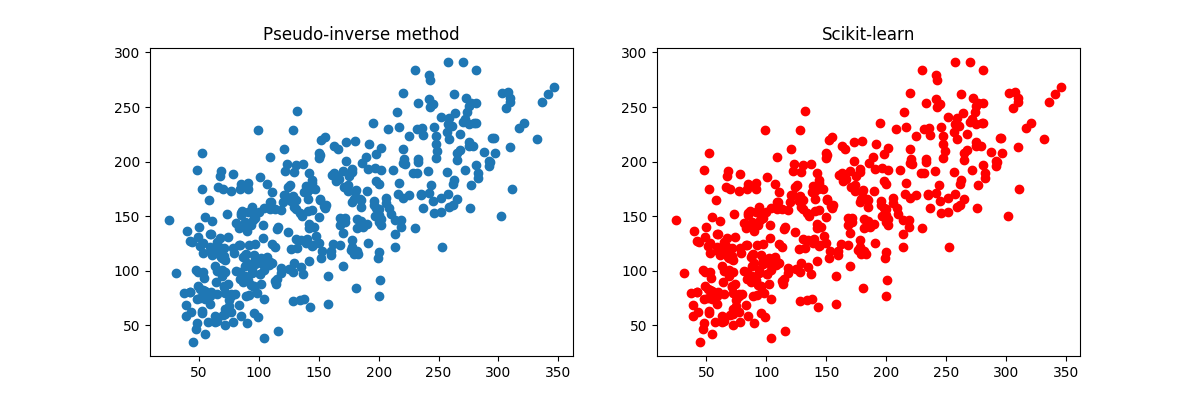
\includegraphics[scale=0.3]{diabetes_accuracy}
\end{center}
Both methods give exactly the same result as can be seen from the identical mean square error.

\section{Regularization}

The gradient of $L_{2}$ regularization can be derived as follow:
\begin{equation}
\begin{split}
	\nabla _aE_{L2} &= \frac{\partial ||f - Ya||^2_2 + \gamma ||a||^2_2}{\partial a}\\
	 &= 2Y^T(f - Ya) + 2\gamma a
\end{split}
\end{equation}
Equating the gradient to 0 gives the closed form of \textit{a} as follow
\begin{equation}
\begin{split}
	0 &= 2Y^T(f - Ya) + 2\gamma a\\
	Y^TYa - \gamma a &= Y^Tf\\
	a(Y^TY - \gamma) &= Y^Tf\\
	a &= (Y^tY - \gamma)^{-1} Y^Tf 
\end{split}
\end{equation}

It can be observed that the coefficients of the predictor with $L_2$ regularization are significantly lower than the model without regularization. This is caused by adding a quadratic penalty of the weights to the error function. The coefficients of the model with and without $L_2$ regularization is shown below.
\begin{center}
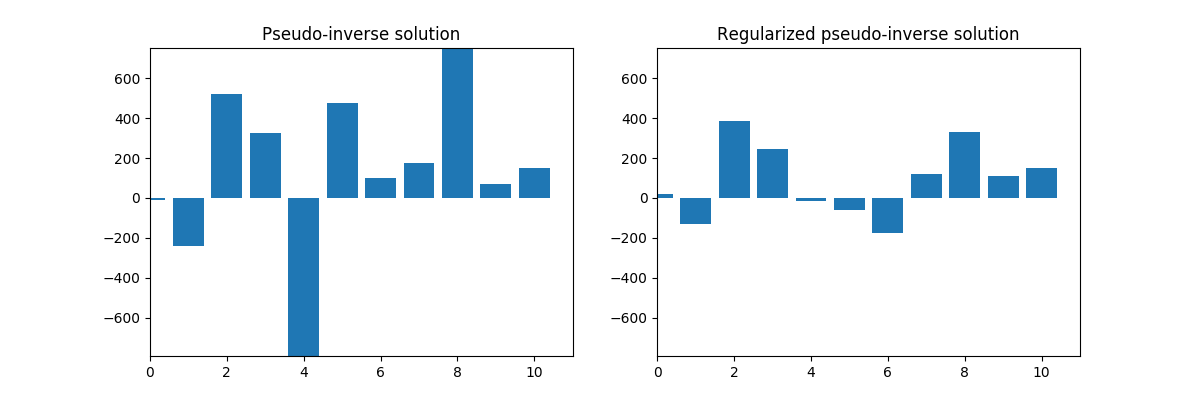
\includegraphics[scale=0.4]{reg_weights_compare}
\end{center}

\section{Sparse Regression}

\section{Solbility Prediction}

\end{document}